\documentclass[main.tex]{subfiles}

\begin{document}



\authors{Eric Burdette and Greg Hirth}
\affiliation{1}{Department of Earth, Environmental and Planetary Sciences, Brown University, Providence, RI, USA}

\begin{keypoints}
\item Antigorite was deformed at two loading rates and subsequently dehydrated
\item Dynamic rupture can be produced with slow ($10^{-5}$) loading and dehydration before samples reach peak strength.
\end{keypoints}


\clearpage
%\section*{Abstract}


\section{Introduction}

\doublespacing %start text

    Subduction zones are among the most seismically active areas on earth. The wide spectrum of brittle and ductile behavior in the nearby mantle and downgoing slab control seismic coupling, deep fluid transport, and mantle convection. The interplay between rheology and metamorphic reactions is key to understanding tectonic dynamics and evolution at depth.\\
    
    Slabs descending into the mantle carry chemically bound liquids in the form of hydrous minerals. Antigorite is an abundant and efficient mineral in the slab to carry this water.  Heating of the slab at depth along the geothermal gradient causes dehydration \citep{Hacker2003}. The subsequent water release is hypothesized to be a cause of dehydration melting that generates arc volcanism, a mechanism for decoupling of the downgoing slab to the convecting mantle, and the source for intermediate depth seismicity. The seismicity is thought to be due to reaction generated pore fluid pressure and velocity feedback on strength in the material \citep{Raleigh1965}, but this is poorly established experimentally at relevant pressures.\\
    
    Several studies at low pressure have showed that antigorite can generate unstable dynamic rupture at pressure below 500 MPa \citep{Raleigh1965, Murrell1976, Reinen1994, Okazaki2015}. However, studies attempting to replicate the unstable behavior at pressure above 500 MPa have not produced acoustic emissions or dynamic rupture \citep{Hilairet2007, Chernak2010, Chernak2011, Proctor2015, Ferrand2017} even when stiffness was reduced by an order of magnitude, which strongly enhances shear weakening and activates shear heating, but slip rates only reach 40 um/s (\cite{burdette2020enhanced}). Why is this?\\
    
\begin{figure}
  \includegraphics[width=\textwidth]{Sections/Appendix1/Figures/Pc_stiffnessPlot.png}
  \caption{Confining pressure and corresponding apparatus stiffness for studies of antigorite dehydration mechanical behavior. D-DIA studies referenced are \cite{Hilairet2007} and \cite{Gasc2011}.  Griggs apparatus studies referenced are \cite{Chernak2011}, \cite{Proctor2015}, and \cite{Okazaki2016}. Gas Rig experiments referenced are \cite{Okazaki2015} and \cite{Murrell1976}.}
  \label{fig:A1_StiffnessvsP}
\end{figure}
    
    Several recent studies focus on 'plastic' deformation mechanisms that allow antigorite to deform without increasing its volume (\cite{Escartin1997, david2020sliding}). This non-dilatant deformation is characterized by distributed shear sliding on mode 2 cracks whose displacement is limited by grain boundaries with sheets of a different orientation. Data from chapter 2 shows the shear cracks at grain boundaries kink the next grain, and can tear it at high strain, generating gouge. In synchrotron studies (\cite{Hilairet2007}), tearing may be the primary deformation mechanism, amorphising more than 40\% of the sample \citep[][figure 6]{amiguet2014deformation}. Low strain, and low strainrate experiments above 400°C (Figure \ref{fig:CH2_All_Antig_microstructure}) show less microcrack damage, however, which implies some recovery of the kinks as well as rotation of grains towards high shear stress orientations (CPO).\\
    
    The contrast in CPO and damage between high and low strain rate experiments sheds light on several unpublished results at low strain rate from our previous investigations gathered here. We were able to produce a dynamic earthquake-like slip event by slowly loading a gouge sample, and increasing temperature to dehydrate it before reaching peak stress. We were also able to produce more rapid slip  deforming a sample loaded quickly, but dehydrated at lower stress before significant plastic deformation occurred (in contrast to peak stress dehydration). A constant stress creep sample which produced a small, but dynamic slip event slightly above antigorite's dehydration temperature illustrates the development of an unstable fault moving through samples.\\


\section{Methods}
    Methods for material preparation and protocols for temperature ramping dehydration experiments are detailed in chapter 1. Methods for material preparation and protocols for stress stepping on solid antigorite cores are detailed in chapter 2. All experiments in this section were conducted at 1 GPa confining pressure and used the modified compliance column \cite{burdette2020enhanced}.
    
\begin{figure}
  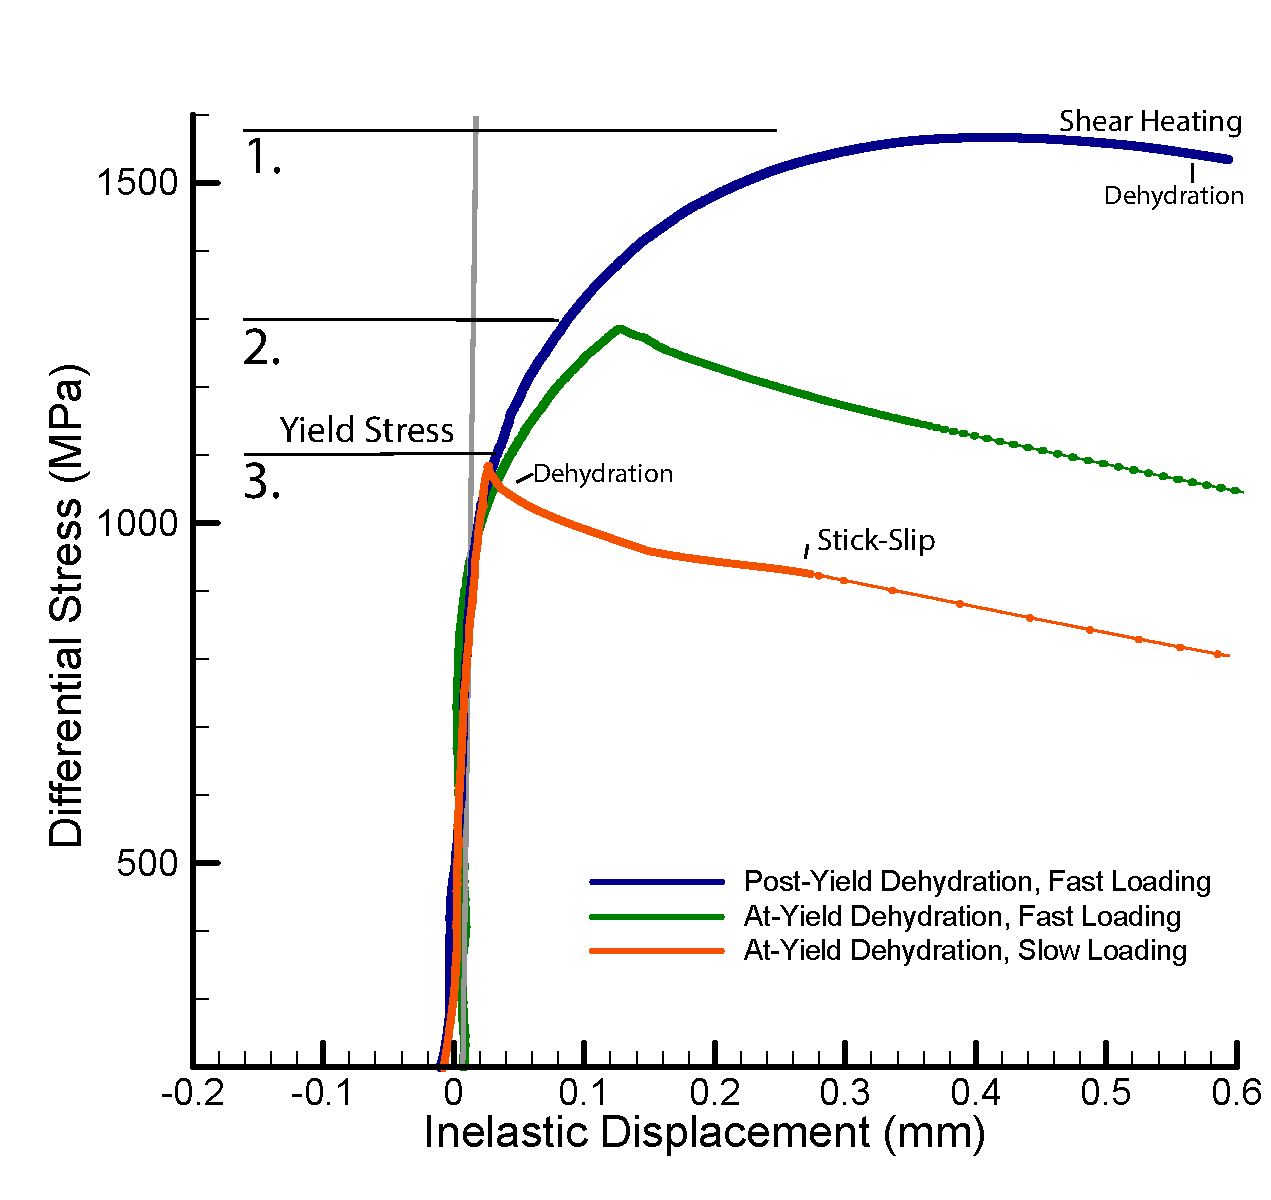
\includegraphics[width=\textwidth]{Figures/Compaction_plan_edit-dots_w2235.pdf}
  \caption{Differential stress and sample displacement are shown for three dehydration experiments at 1 GPa confining pressure. The first is and experiment from previous work that was allowed to reach peak stress ("Shear Heating") before dehydrating loaded 'Fast' ($10^{-4} 1/s$), The second is and experiment loaded 'Fast', but dehydrated before reaching peak stress, and the third is an experiment loaded "slowly" ($10^{-5} 1/s$) and also dehydrated before reaching yield ("Stick-Slip").  Labels indicate time of dehydration. Numbered stress levels indicate peak stress for each experiment. Points are plotted at 1 Hz recording rate}
  \label{fig:A1_Stress-strain_yieldingDehydr}
\end{figure}

\begin{figure}
  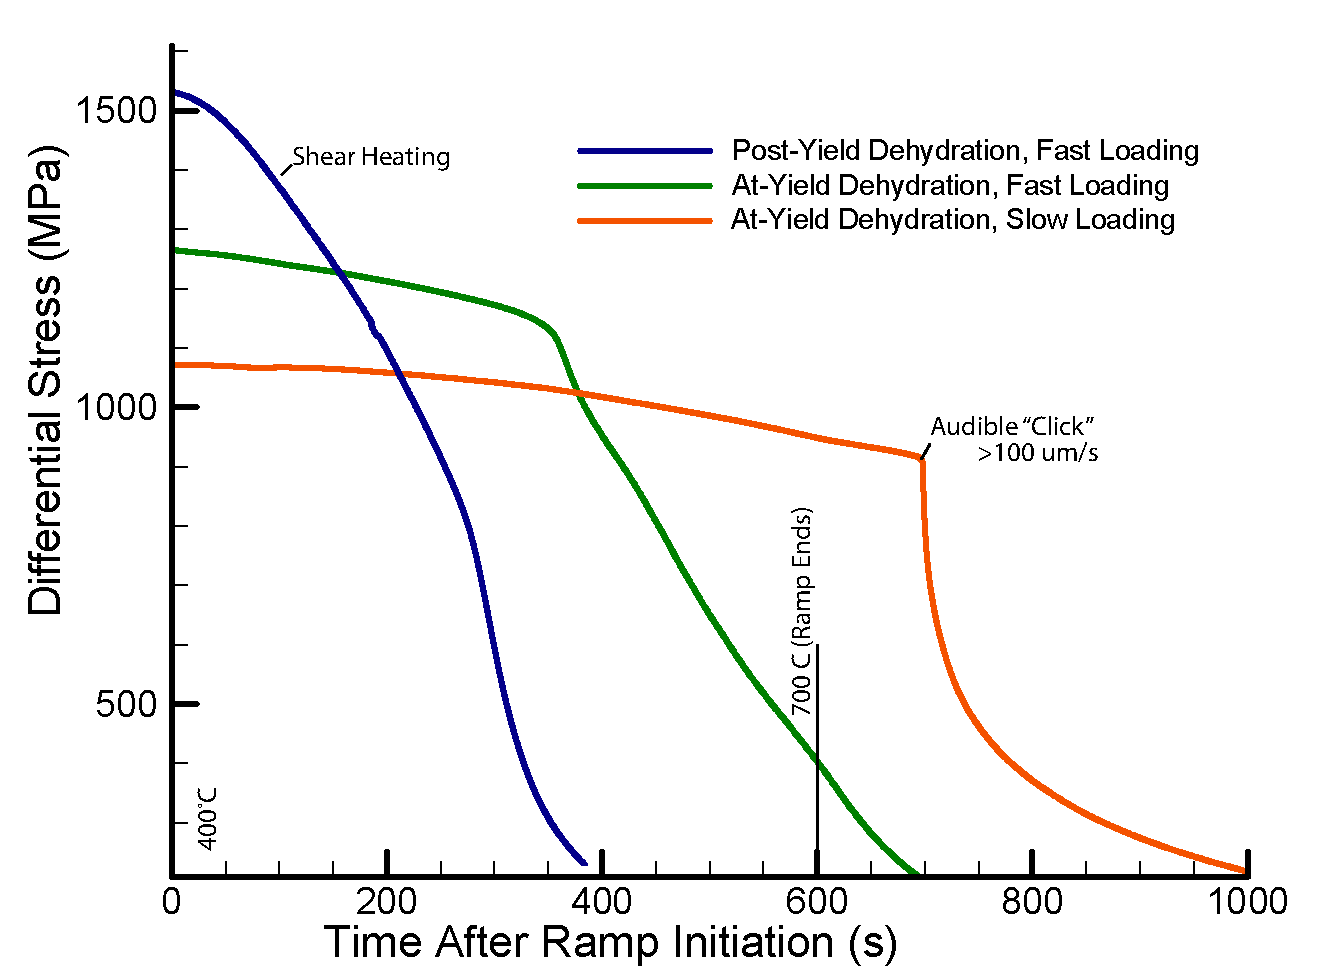
\includegraphics[width=\textwidth]{Figures/Pre-Yield_Comparison_w2235added.pdf}
  \caption{Load-time data from shear heating (post-yield dehydration), and preliminary stick-slip runs (pre-yield dehydration). Temperature was ramped from 400 \(^o\)C to 700 \(^o\)C over 600 seconds to initiate dehydration. Sample displacement speed is noted for the pre-yield run at the time when stick-slip occurred.}
  \label{fig:A1_Stress-time_yieldingDehydr}
\end{figure}

\section{Results}
    \subsection{Mechanical Data}
        Mechanical data were collected for several dehydration experiments at 1 GPa, where loading displacement rate and strain at which dehydration was initiated varied (figure \ref{fig:A1_Stress-time_yieldingDehydr}, figure \ref{fig:A1_Stress-strain_yieldingDehydr}). Results of dehydration at peak stress with "fast" (1.8 um/s) loading are discussed in detail in chapter 1. The dehydration completes in 400 seconds before the furnace has reached 700°C, and peak displacement rate is 40 um/s. The displacement during dehydration is very large (10 mm) which activates shear heating.
        
        An intermediate experiment, where the sample was dehydrated before reaching peak stress with "fast" loading, is also displayed. It weakens more slowly, finishing around the 600 second time when the furnace reaches 700°C. Its peak displacement rate is 15 um/s, and shows no signs of stick-slip activity.
        
        In a final experiment (and repeat), samples were loaded "slowly" (0.18 um/s) and dehydrated before yield. The samples do not weaken substantially during the ramp of furnace temperature to 700°C. Shortly after reaching 700°C, the samples slip rapidly at speeds greater than 100 um/s, and weakens 500 MPa in 50 seconds.
        
        Stress-stepping creep data for the dehydrating antigorite creep is discussed in section \ref{ch2_620}. After 7 hours at temperature (620°C), a small stick-slip event occurred, generating a fault running partway through the sample. Only two subsequent load steps were completed to prevent further deformation from overprinting the fault.
\begin{figure}
  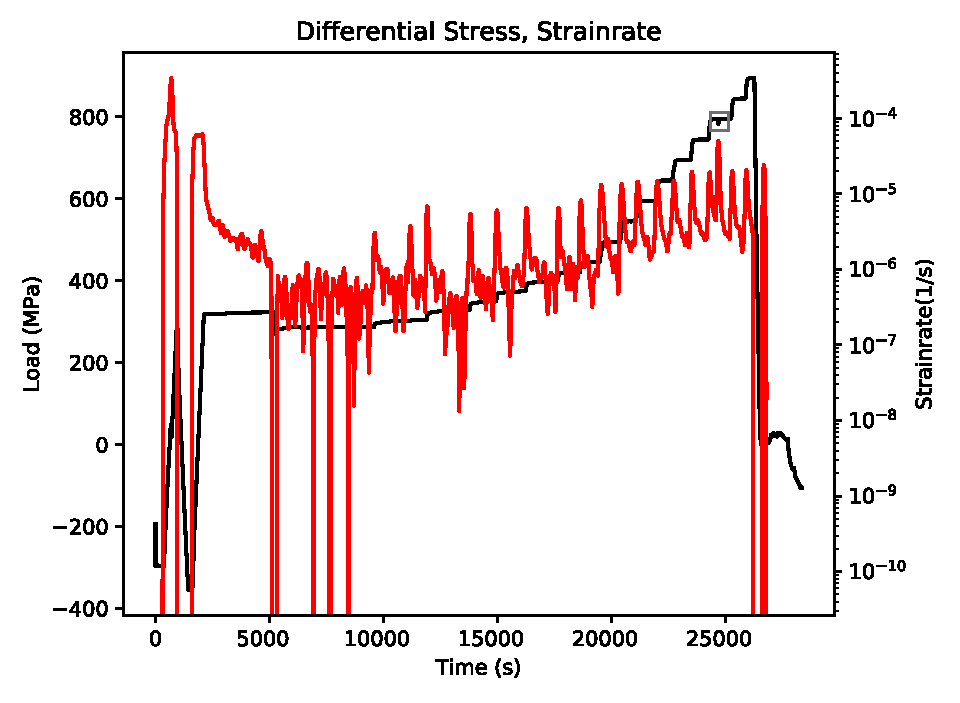
\includegraphics[width=\textwidth]{Figures/W2446_Stress-Strainrate-time.pdf}
  \caption{Load-strainrate-time data from creep experiment W2446. The sample creeps at rates above $10^{-7}$ 1/s even at a stress of 500 MPa. Note the late stick-slip event outlined in grey.}
  \label{fig:A1_Stress-Strainrate-time_W2446}
\end{figure}

\begin{figure}
  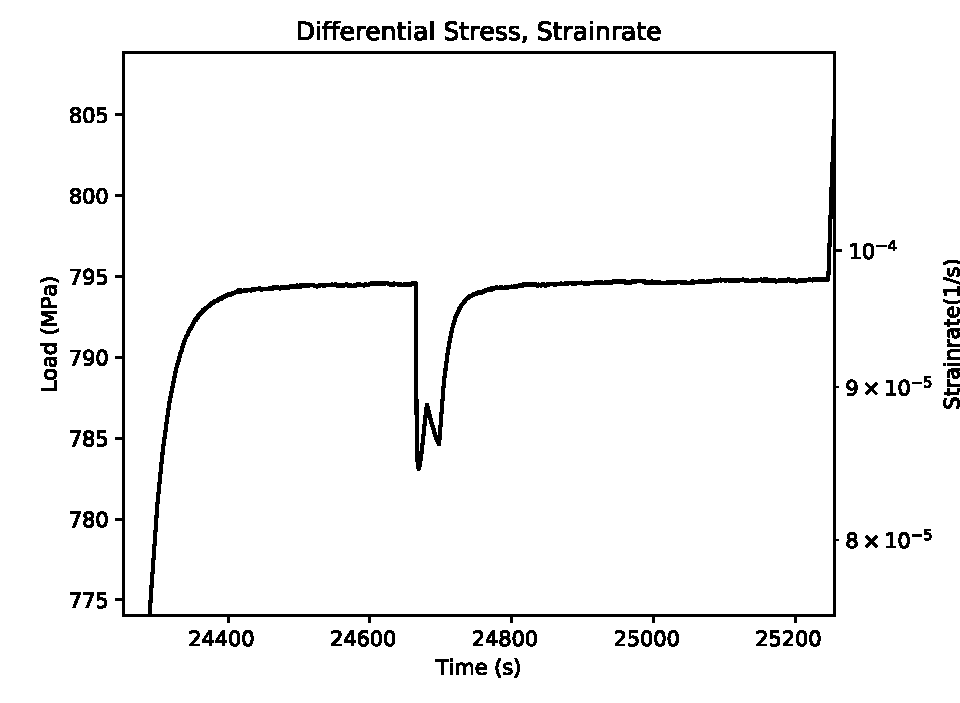
\includegraphics[width=\textwidth]{Figures/W2446_Stress-Strainrate-time Zoom.pdf}
  \caption{Load-time data showing the rapid stick-slip event in experiment W2446. The 12 MPa load drop happens in a single sample interval at 10Hz recording rate. Corresponding microstructure and a relict fracture is shown in figure \ref{fig:A1_Creep_W2446_collage}}
  \label{fig:A1_Stress-Strainrate-time_W2446_zoom}
\end{figure}        
        
    \subsection{Microstructure}
        Microstructure for the sample dehydrated at peak load has several unique characteristics. First, reaction products are clearly visible in most parts of the sample, with high contrast (bright) olivine grains decorating fractures, pore space, and the highly reacted fault core. There is a clear gradient in reaction extent from the center of the deformed fault core where the antigorite has fully reacted to the shear piston surfaces, where reaction products are barely visible in intergranular porosity. Circular pores are present in the fault core which were presumably water-filled in-situ. The fault zone is relatively wide, with more than 200 um of its 1200 um thickness fully reacted after 10 mm of slip (Figure \ref{fig:S5}). Outside the fault zone, alignment of grains is poor, and a number of secondary fractures cross the sample in the R1 orientation. No kinking of the grains is preserved either inside or outside the fault core.
        
        The second sample, also ramped to stress "fast" ($10^{-4} 1/s$), but dehydrated early before reaching peak stress, has pore space remaining throughout the sample. In contrast to the peak stress dehydration, there are fewer fractures, and less damage. Reaction extent is much lower, with reaction products mostly visible filling small (sub-micron) shear fractures. Faults are still relatively rough, with many antigorite grains torn and bent at the fault surfaces, and little plasticity outside the multiple 2um wide fault traces. 
        
        The sample ramped "slowly" ($10^{-5} 1/s$) and dehydrated early has little pore space remaining, and a single narrow ($~1 \mu m$) fracture running through its length (figure \ref{fig:A1_Full_Sample_Compare}). Porosity is not visible between grains. Antigorite grains $>10 \mu m$ from the fault surface are clearly plastically deformed, with kinks and bent grains visible. Near the fault surface deformation is more intense, with some grains displaying kink angles greater than 45 degrees. Despite this plasticity, the fracture appears very smooth (figure \ref{fig:A1_W2296_FaultZoom}). There is evidence of reaction on the fault, but it only extends 3 um from the fault surface. These features roughly match the fault developed in a dehydrating creep experiment.
        
\begin{figure}
  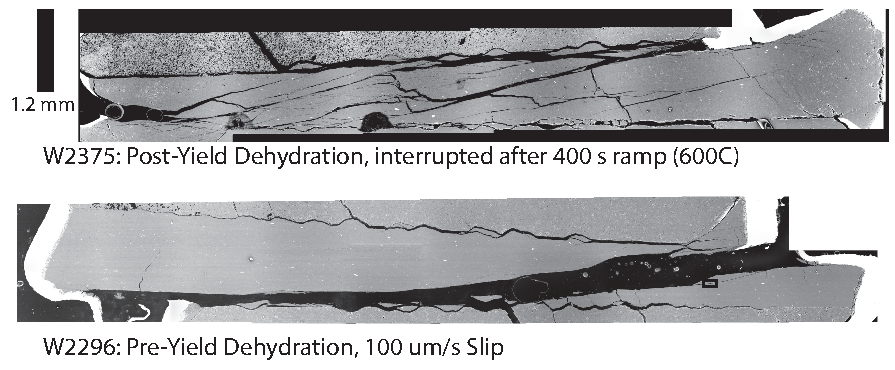
\includegraphics[width=\textwidth]{Figures/Full Sample_W2375vsW2296.pdf}
  \caption{Broad microstructure comparison of a sample loaded to peak stress, dehydrated, then interrupted partway through the dehydration temperature ramp and a sample dehydrated before yielding. Note differences in damage and faulting.}
  \label{fig:A1_Full_Sample_Compare}
\end{figure}

        The creep experiment run at 620°C is a cored sample of mesh-textured antigorite, so the sample started with very low permeability and porosity, and no visible damage. The sample recovered after deformation has a single large fracture oriented 35 degrees to the compression axis. Offset on the fault matches the 200 um slip event recorded during deformation. The fault trace is jagged, with some smooth sections, apparently fractured along the grain boundaries of antigorite. Several sections of the fault rupture through grains of antigorite whose basal planes were oriented perpendicular to the fault surface. These poorly oriented grains are bent over and torn into sub-micron particles that fill short sections of the fault and have high backscatter contrast (bright) suggesting they are reacting due to the increased surface area.

\section{Discussion}
    \subsection{Overcoming Anisotropic Toughness}
        An unusual feature of sheet silicate deformation at high pressure is the dominance of shear cracking and linkage over dilatant wing crack bridging that causes failure in other brittle rocks. One might expect that shear crack bridging would generally be easier, but antigorite can reach strengths 1/2 those of granites  at 1 GPa. Antigorite's strength comes from its structure and unique mesh textures, where grains are often oriented with basal planes perpendicular to adjacent grains. Shear cracks would need to take multiple long 90 degree jogs, or penetrate through sheets of adjacent grains to bridge with other nearby cracks. When tested at room pressure, this structure gives antigorite unusually high tensile strength among rocks \citep[][\ via Brazilian tensile tests]{david2020sliding}, demonstrating the toughening effect the mesh texture contributes.
        
        In-situ, the shear cracks impinging on perpendicular grains results in kinks, whose structures are discussed in chapter 2. At high strains, instead of tearing and sliding through the poorly oriented grains, new kinks form elsewhere in samples at high confining pressures. This results in highly distributed deformation in high shear stress orientations (Chapter 2, figure \ref{fig:CH2_All_Antig_microstructure}).
        
        At the 550°C in creep experiments, very few kinks are recovered and grains appear "bent" and rotated from their original orientation with no additional porosity appearing. It is easy to imagine how a stress-concentrating feature could generate an aligned strain localized zone above 550°C if it were given enough time to propagate through the sample. The fact that ductile features do not dominate previous experiments at this temperature \citep{Chernak2010, Proctor2016} suggests that there is still some hardening that occurs, and if driven at "fast" strain rates the samples will tear grains to form a brittle fault along alignment set up during loading.
\begin{figure}
  \includegraphics[width=\textwidth]{Figures/W2446_Fault_collage.pdf}
  \caption{a) SEM image of dehydrating creep sample W2446. Sub-image locations are noted by black boxes. b) Image of a rough fault section where poorly aligned grains are torn and bent back to form fault gouge. c) smooth section of the fault with no grains penetrating into the fault core and no visible gouge.}
  \label{fig:A1_Creep_W2446_collage}
\end{figure}

\begin{figure}
  \includegraphics[width=\textwidth]{Figures/W2296_zoom_006.jpg}
  \caption{SEM Image of reaction on the smooth fault surface from pre-yield experiment W2296. Location is noted in larger Figure \ref{fig:A1_Full_Sample_Compare}}
  \label{fig:A1_W2296_FaultZoom}
\end{figure}        
        
    \subsubsection{Brittle-Ductile Path and Rate Dependence}
        The series of experiments here describe a path through the brittle-ductile transition in antigorite that preserves/promotes what could be key elements for dynamic slip of antigorite: low permeability and localization. 
        
        At high strain rates, gouge experiments have very little time to close porosity and linked permeable paths. After yielding samples harden towards peak stress, tearing grains and opening paths between existing porosity. In addition, the hardening promotes distribution of deformation around a fault, instead of strong localization onto a single fault. The large amount of stored energy (+50\%) at peak stress with a large amount of ground, amorphous antigorite gouge in the fault core contributes to rapid pore-fluid pressure weakening and shear heating as slip progresses to high strain (figure \ref{fig:A1_Stress-time_yieldingDehydr}). This structure is unlikely to exist in nature.
        
        If gouge samples are ramped to stress "fast" but not loaded to peak stress, deformation does not distribute onto a wide fault core, but instead onto several narrow faults. The fast ramping to stress does not allow time to align sheets or close pores so permeability remains high. The stored energy in the machine is lower at lower starting stress for dehydration, and it lacks gouge to react quickly so it weakens more slowly and still does not generate rapid slip events.
        
        When gouge samples are ramped to stress "slowly" and not loaded to peak stress, porosity/permeability normal to the fault closes and grains align to localize deformation onto a single narrow fault. The extra time to accommodate plastic deformation (several hours) allows this difference. There is very little deformation during the temperature ramping period due to the more cohesive nature of the sample, without gouge and porosity to generate significant early reaction products. Shortly after the sample reaches 700°C the smooth fault suddenly and rapidly slips, generating the small amount of observed reaction products on the fault surfaces. The very small amount of reaction products from high slip speed (in comparison to the sample ramped at peak stress) suggests the fault weakens very efficiently compared to the sample ramped at peak stress.
        
    \subsection{Natural Context}
        Natural antigorite bodies sit for very long times at low stress in subduction zones. If their microstructural development is similar to that described above, they are most likely to behave like the slowly loaded dehydration or creep samples, developing strongly localized faults with anisotropic permeability. When these faults approach dehydration temperatures, they could rupture generating dynamic earthquake events like those we observe in the lab.
        
        
\section{Conclusion}
    We deformed antigorite gouge and isotropic cores along three loading/creep paths and observed their weakening behavior. Samples loaded "fast" to peak stress weakened quickly due to high reaction rates in their distributed, amorphized fault cores. Samples loaded "fast" and dehydrated before peak stress weaken/react more slowly, with several active faults accommodating deformation and little shear heating activity.  Samples loaded "slowly" and dehydrated before peak stress had the least visible porosity and damage, with deformation localized onto a single fault which dynamically ruptured after very little weakening. These results together suggest further laboratory investigations of dehydration embrittlement should be conducted over long times on samples with mature, compacted faults. Natural faults are most like the "slow" path, potentially resolving a longstanding mystery around the apparent rate-strengthening behavior coexisting with dehydration embrittlement.


\singlespacing % back to single spaced






\clearpage

\end{document}
 